\section{Descripción y caracterización detallada del problema}

\subsection{Criterios y proceso de selección del problema}

A partir de los tres problemas identificados en la Introducción, se realizó un proceso de comparación para seleccionar un problema con alto impacto social, urgencia evidente y viabilidad técnica para un prototipo de IA dentro del tiempo del curso. La selección se basó en los siguientes criterios:

\begin{enumerate}
	\item \textbf{Impacto social medible:} afecta directamente a pacientes (especialmente crónicos) y se refleja en deterioro de continuidad de tratamientos y quejas/tutelas.
	\item \textbf{Urgencia temporal:} crisis activa que requiere medidas de apoyo en el corto plazo.
	\item \textbf{Viabilidad técnica con IA (MVP):} posibilidad de construir un flujo completo y evaluable con OCR, KNN y fuentes de datos disponibles.
	\item \textbf{Disponibilidad de datos:} existencia de fuentes públicas u oficiales para construir un catálogo mínimo (p.\ ej., INVIMA y MinSalud).
	\item \textbf{Factibilidad de implementación:} implementación de software realizable en el marco del proyecto académico.
	\item \textbf{Empoderamiento del usuario:} entrega información práctica directamente al paciente.
	\item \textbf{Escalabilidad:} capacidad de crecimiento a más medicamentos y más fuentes.
\end{enumerate}

\subsubsection{Comparación entre los problemas identificados}

\begin{itemize}
	\item \textbf{Problema 1: Desabastecimiento de medicamentos y falta de alternativas.} Presenta impacto directo en la continuidad del tratamiento y permite un MVP con un flujo claro: foto del empaque $\rightarrow$ identificación por OCR $\rightarrow$ alternativas por principio activo. Además, su evaluación es viable (acierto de mapeo y coherencia de alternativas).
	
	\item \textbf{Problema 2: Ineficiencia en la gestión de inventarios farmacéuticos.} Aunque tiene gran impacto sistémico, suele requerir datos operativos internos (inventarios, compras, distribución) y acuerdos con actores de la cadena, lo cual dificulta un prototipo realista en el tiempo del curso.
	
	\item \textbf{Problema 3: Asimetría de información entre pacientes y el sistema de salud.} Es relevante, pero su alcance es amplio (precios, disponibilidad, regulación, comparativos). Parte de esta brecha informativa se reduce abordando el Problema 1, ya que MediFinder entrega información y alternativas de manera directa al usuario.
\end{itemize}

Con base en esta comparación, se seleccionó el \textbf{Problema 1} por maximizar impacto en el paciente y ofrecer una ruta técnica clara, evaluable y escalable dentro del marco del curso.

\subsection{Caracterización detallada del problema seleccionado}

La Universidad Javeriana señala que el asunto no reside únicamente en la ausencia física de medicamentos, sino en fallas en el abastecimiento y la cadena asociadas a la crisis financiera del sistema \cite{diaz2025}.

La falta de abastecimiento y entrega de medicamentos no solo afecta a los pacientes sino también a hospitales. Durante el año pasado, por suspensión de actividades de empresas productoras a nivel nacional, el Ministerio de Salud reportó escasez de fármacos vitales como norepinefrina o vasopresina (usados principalmente en UCI). En el caso de la norepinefrina, el mercado está cubierto en un 26\% por Laboratorios Ryan con 120.000 ampollas mensuales entre septiembre y diciembre; sin embargo, dicha cantidad no ha sido suficiente para cubrir la demanda, motivo por el cual el medicamento permanece en la lista de vital no disponible desde 2018 \cite{saavedra2025}.

Debido a esto, se otorgaron licencias y autorizaciones de importación a empresas externas. Empresas como Holland Group, Pisa Farmacéutica, Reprefarco y Sicmafarma facilitaron la llegada de unidades importadas; por ejemplo, se reportaron aproximadamente 100.000 unidades a través de Reprefarco, además de aportes de Nextpharmasourcing, lo cual incrementa costos en un contexto de crisis \cite{saavedra2025}.

Asimismo, a pesar de que se incrementa el desembolso de los colombianos en compra de medicamentos, esto no garantiza acceso oportuno. Persisten demoras extensas, faltantes y alzas en precios, generando inconformidad entre población dependiente de tratamientos (enfermedades crónicas, patologías huérfanas o tratamientos de alto costo) \cite{calero2025}.

\begin{figure}[H]
	\centering
	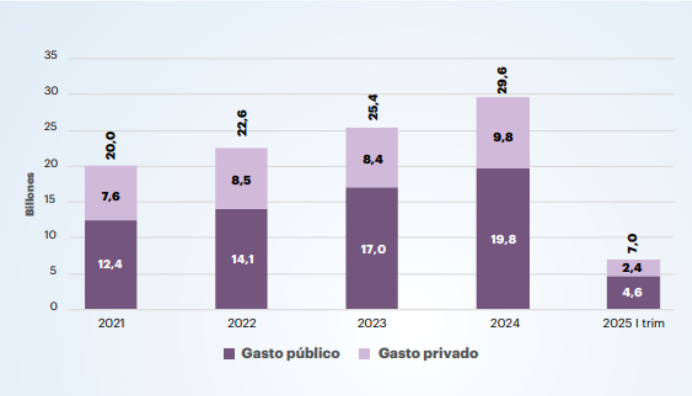
\includegraphics[width=0.90\textwidth]{img/gasto.png}
	\caption{Detalle del gasto en salud por categorías 2021-2025}
	\label{fig:gasto}
\end{figure}

\begin{figure}[H]
	\centering
	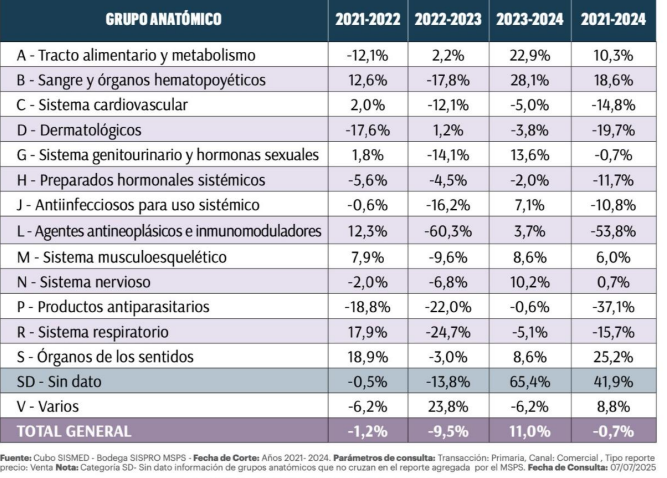
\includegraphics[width=0.85\textwidth]{img/evolucionGasto.png}
	\caption{Evolución del gasto privado en medicamentos en Colombia 2021-2025}
	\label{fig:evolucion}
\end{figure}

Como se evidencia en las gráficas anteriores, el gasto privado en salud aumentó en los últimos años, pasando de 20 billones a 29.2 billones entre 2021 y 2024, con un aumento nominal del 48.0\% y del 13.8\% después de inflación \cite{acemi2025}.

Igualmente, el gasto en medicamentos no incluye costos adicionales asociados a la gestión para la disposición de medicinas en gestores farmacéuticos o prestadores de servicios de salud \cite{acemi2025}.

En síntesis, la problemática es compleja y de alcance nacional. Sin embargo, la espera por soluciones estructurales puede dejar a los pacientes expuestos a interrupciones de tratamiento. En este contexto, una herramienta tecnológica de apoyo, basada en IA, puede ofrecer alternativas temporales e información útil al usuario mientras se estabiliza el sistema.

\pagebreak